\documentclass[12pt, a4paper, oneside]{article}\usepackage[]{graphicx}\usepackage[]{color}
%% maxwidth is the original width if it is less than linewidth
%% otherwise use linewidth (to make sure the graphics do not exceed the margin)
\makeatletter
\def\maxwidth{ %
  \ifdim\Gin@nat@width>\linewidth
    \linewidth
  \else
    \Gin@nat@width
  \fi
}
\makeatother

\definecolor{fgcolor}{rgb}{0.345, 0.345, 0.345}
\newcommand{\hlnum}[1]{\textcolor[rgb]{0.686,0.059,0.569}{#1}}%
\newcommand{\hlstr}[1]{\textcolor[rgb]{0.192,0.494,0.8}{#1}}%
\newcommand{\hlcom}[1]{\textcolor[rgb]{0.678,0.584,0.686}{\textit{#1}}}%
\newcommand{\hlopt}[1]{\textcolor[rgb]{0,0,0}{#1}}%
\newcommand{\hlstd}[1]{\textcolor[rgb]{0.345,0.345,0.345}{#1}}%
\newcommand{\hlkwa}[1]{\textcolor[rgb]{0.161,0.373,0.58}{\textbf{#1}}}%
\newcommand{\hlkwb}[1]{\textcolor[rgb]{0.69,0.353,0.396}{#1}}%
\newcommand{\hlkwc}[1]{\textcolor[rgb]{0.333,0.667,0.333}{#1}}%
\newcommand{\hlkwd}[1]{\textcolor[rgb]{0.737,0.353,0.396}{\textbf{#1}}}%

\usepackage{framed}
\makeatletter
\newenvironment{kframe}{%
 \def\at@end@of@kframe{}%
 \ifinner\ifhmode%
  \def\at@end@of@kframe{\end{minipage}}%
  \begin{minipage}{\columnwidth}%
 \fi\fi%
 \def\FrameCommand##1{\hskip\@totalleftmargin \hskip-\fboxsep
 \colorbox{shadecolor}{##1}\hskip-\fboxsep
     % There is no \\@totalrightmargin, so:
     \hskip-\linewidth \hskip-\@totalleftmargin \hskip\columnwidth}%
 \MakeFramed {\advance\hsize-\width
   \@totalleftmargin\z@ \linewidth\hsize
   \@setminipage}}%
 {\par\unskip\endMakeFramed%
 \at@end@of@kframe}
\makeatother

\definecolor{shadecolor}{rgb}{.97, .97, .97}
\definecolor{messagecolor}{rgb}{0, 0, 0}
\definecolor{warningcolor}{rgb}{1, 0, 1}
\definecolor{errorcolor}{rgb}{1, 0, 0}
\newenvironment{knitrout}{}{} % an empty environment to be redefined in TeX

\usepackage{alltt} % Paper size, default font size and one-sided paper
%\graphicspath{{./Figures/}} % Specifies the directory where pictures are stored
%\usepackage[dcucite]{harvard}
\usepackage{rotating}
\usepackage{amsmath}
\usepackage{setspace}
\usepackage{pdflscape}
\usepackage[flushleft]{threeparttable}
\usepackage{multirow}
\usepackage[comma, sort&compress]{natbib}% Use the natbib reference package - read up on this to edit the reference style; if you want text (e.g. Smith et al., 2012) for the in-text references (instead of numbers), remove 'numbers' 
\usepackage{graphicx}
%\bibliographystyle{plainnat}
\bibliographystyle{agsm}
\usepackage[colorlinks = true, citecolor = blue, linkcolor = blue]{hyperref}
%\hypersetup{urlcolor=blue, colorlinks=true} % Colors hyperlinks in blue - change to black if annoying
%\renewcommand[\harvardurl]{URL: \url}
\IfFileExists{upquote.sty}{\usepackage{upquote}}{}
\begin{document}
\title{Exam Answers}
%\author{Rob Hayward\footnote{University of Brighton Business School, Lewes Road, Brighton, BN2 4AT; Telephone 01273 642586.  rh49@brighton.ac.uk}}
\date{\today}
\maketitle
\section*{Question 1}
\subsection*{a}
\begin{align*}
Q_d =& 800 - 7p\\
Q_d =& 800 - 7 \times 10\\
Q_d =& 800 - 70\\
Q_d =& 730
\end{align*}

\subsection*{b}
At the equilibrium $Q_d = Q_s$, therefore
\begin{align*}
Q_d = 800 - 7p =& 50 +8p = Q_s\\
800 - 7p =& 50 + 8p\\
800 -50 =& 8p + 7p\\
750 =& 15p\\
\frac{750}{15} =& p\\
50 =& p
\end{align*}
When p = 50, 
\begin{align*}
Q_d =& 800 - 7 \times 50\\
Q_d =& 800 - 350\\
Q_d =& 450
\end{align*}

\subsection*{c}
We know that the equilibrium price is above the price ceiling of 40.
The quantity demanded
\begin{align*}
Q_d =& 800 - 7 \times 40\\
Q_d =& 800 - 280\\
Q_d =& 530
\end{align*}
The quantity supplied
\begin{align*}
Q_s =& 50 + 8 \times 40\\
Q_s =& 50 + 320\\
Q_s =& 370
\end{align*}

Demand is greater than supply.  There will be an attempt to break the ceiling.  

\begin{knitrout}
\definecolor{shadecolor}{rgb}{0.969, 0.969, 0.969}\color{fgcolor}
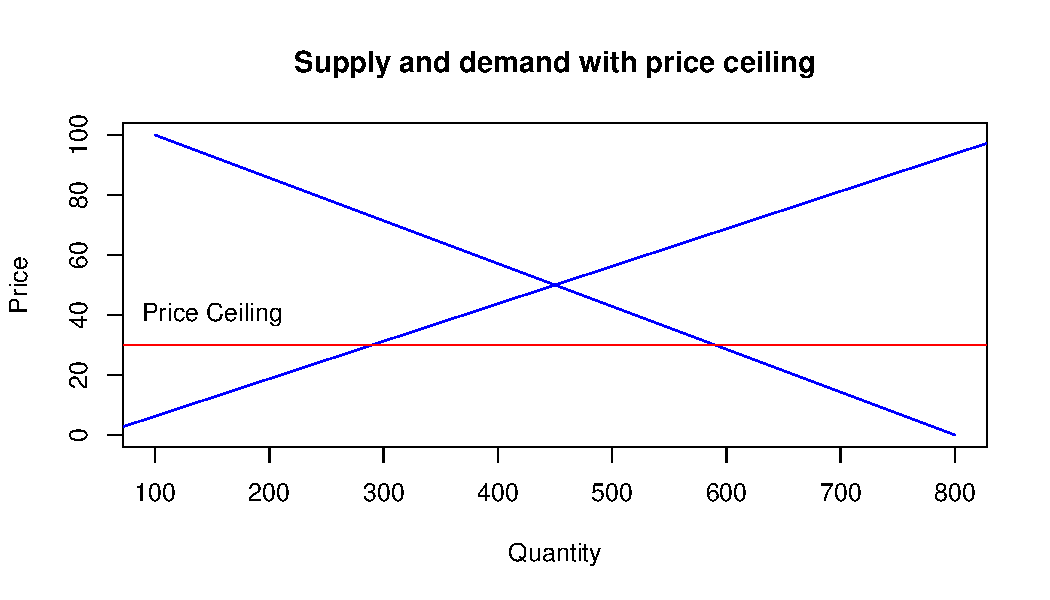
\includegraphics[width=\maxwidth]{figure/ceiling} 

\end{knitrout}

\subsection*{d}
Now
\begin{align*}
Q_d = Q_s = 500 -& 7p = 50 + 8p\\
500 - 50 =& 15p\\
\frac{450}{15} =& p\\
30 =& p
\end{align*}
and 
\begin{align*}
Q_d =& 500 - 7 \times 30\\
Q_d =& 500 - 210\\
Q_d =& 290
\end{align*}

\section{Question 2}
\subsection*{a}
For the standard percentage change method of elasticity. 
\begin{align*}
P_{ed} =& \frac{\% \Delta Q}{\% \Delta P}\\
=& \frac{(6000-10000)/10000}{(12-8)/8}\\
=& \frac{-0.4}{0.5}\\
=& -0.8
\end{align*}
For the mid-point method of elasticity
\begin{align*}
P_{ed} =& \frac{\Delta Q/\text{mid-point} Q}{\Delta P/ \text{midpoint{P}}}\\
=& \frac{(6000-10000)/8000}{(12-8)/10}\\
=& \frac{-4000/8000}{4/10}\\
=& \frac{-0.5}{0.4}\\
=& -1.25
\end{align*}

The advantage of the mid-point method is that it does not change when moving up or down the curve.  

\subsection*{b}
The point elasticity of demand is taken from  
\begin{align*}
P_{ed} = \frac{\Delta Q/Q}{\Delta P /P}
\end{align*}
Re-arrange
\begin{align*}
P_{ed} = \frac{P}{Q} \times \frac{\Delta Q}{\Delta P}
\end{align*}

Therefore, for this question. Where $P = 28$, 
\begin{align*}
Q_d =& 546 - 7 \times p\\
 =& 546 - 7 \times 28\\
=& 546 - 196\\
=& 350
\end{align*}


From the equation for a straight line, $\frac{\Delta Q}{\Delta P}$ is equal to 7. 
Therefore, 
\begin{align*}
P_{ed} =& \frac{28}{350} \times 7\\
=& 0.08 \times 7\\
=& 0.56
\end{align*}


\subsection*{c}
One of the factors that can shift the supply or demand curves is price expectation. Therefore, from equilibrium $1$, the expectation of price decline leads to a left-ward shift of the demand curve for equilibrium $2$ and a right-ward shift of the supply curve to $3$.  This is de-stabilising speculation.

\begin{knitrout}
\definecolor{shadecolor}{rgb}{0.969, 0.969, 0.969}\color{fgcolor}
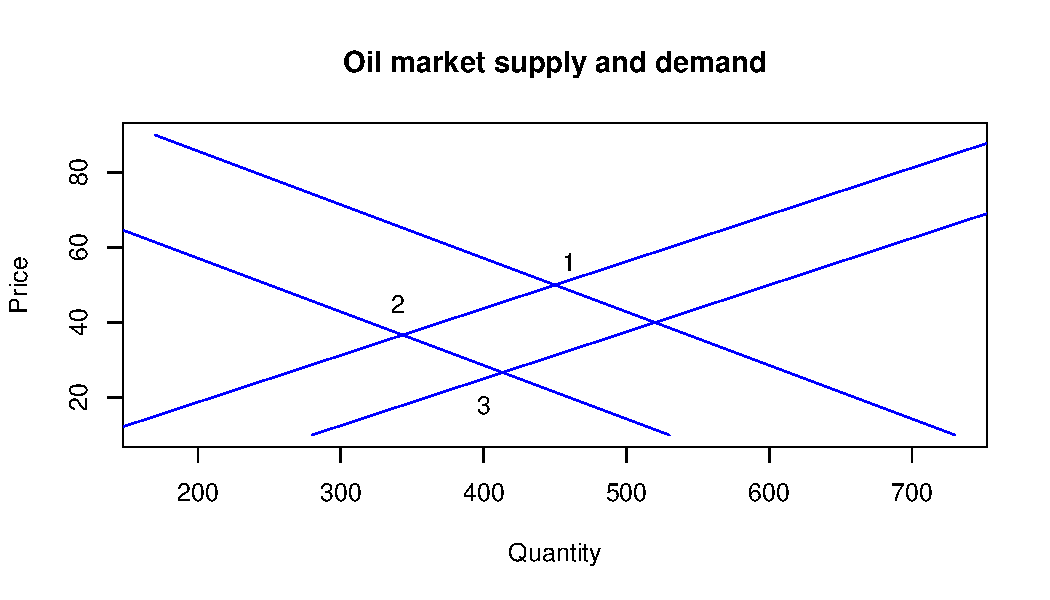
\includegraphics[width=\maxwidth]{figure/speculation} 

\end{knitrout}

\section*{Question 3}
\subsection*{a}
The budget can be used to purchase $\frac{400}{20} = 20$ units of product X or $\frac{400}{16} = 25$ units of product Y.  Therefore, the budget line runs from 20 on the x axis for product X to 25 on the y axis for product Y, forming a tangent to $IC_4$.  The point of tangency must be marked to show the optimum combination of x and y that can be purchased with this budget. 

\subsection*{b}
The slope of the budget line is $\frac{25}{20} = 1.25$ at the original prices.  When the price of good x rises to 40, it is possible to purchase $\frac{400}{40} = 10$ units and the ratio of prices and the slope of the budget line shifts to $\frac{25/10} = 2.5$.  

\subsection*{c}
The budget line will now run from $10$ on the x axis to $25$ on the y axis and will form a tangent to $IC_2$.  The point needs to be shown to get the marks.

\subsection*{d}
Point Z is feasible but it is not optimal.  Utility can be increased by moving from $IC_1$ to $IC_2$.  The curve $IC_5$ cannot be achieved with the current budget.  It would require increased income to push the budget line to the right or a reduction in prices to achieve this level of utility. 

\section*{Question 4}
\subsection*{a}
If total utility is
\begin{align*}
TU = 5X - 4X^2
\end{align*}

Marginal Utility is the derivative 
\begin{align*}
\frac{dU}{dX} = 5 - 8X
\end{align*}

There is diminishing marginal utility because as X increases marginal utility falls.

\subsection*{b}
Given $TPP = 120Q +27Q^2 -Q^3$, the maximum will be when the marginal is zero. Therefore, 

\begin{align*}
\frac{dTPP}{dQ} = 120 + 54Q - 3Q^2 =& 0\\
3Q^2 - 54Q -120 =& 0\\
(3Q - 60)(Q + 2) =&0
\end{align*}

Therefore, either $3Q -60 = 0$ or $Q + 2 = 0$.  In the first case $Q = \frac{60}{3} = 20$, in the second $Q = -2$.  The maximum must be 20. 

\subsection*{c}
Given $TR = 500Q - 5Q^2$, marginal revenue is the derivative. 
\begin{align*}
\frac{dTR}{dQ} = 500 - 10Q
\end{align*}
Given $TC = 20 +20Q +Q^2$, marginal cost is the derivative
\begin{align*}
\frac{dTC}{dQ} = 20 +2Q
\end{align*}
Profit maximisation is when MR = MC, therefore
\begin{align*}
MR = 500 - 10Q =& MC = 20 +2Q\\
500 - 10Q =& 20 +2Q\\
500 - 20 =& 2Q + 10Q\\
480 =& 12Q\\
\frac{480}{12} =& Q\\
40 =& Q
\end{align*}

\subsection*{d}
Total Profit (TP) equals TR - TC, therefore it is equal to 
\begin{align*}
TP =& 500Q - 5Q^2 - 20 -20Q - q^2\\
=& 480Q -6Q^2 -20
\end{align*}

At the maximum output of 40Q.
\begin{align*}
TP =& 480 \times 40 - 6 \times 40^2 - 20\\
=& 19200 - 6 \times 1600 - 20\\
=& 19200 - 9600 - 20\\
=& 9600 - 20\\
=& 9580
\end{align*}

\end{document}
